\graphicspath{{chapters/chapter2/img/}}

\chapter{Data collection}
\label{cha:data}
The dataset used for the project is the echen102/COVID-19-TweetIDs GitHub repository~\cite{chen2020tracking}. The repository contains an ongoing collection of tweet IDs starting on the 28th of January 2020.

The IDs in the dataset are either tweets posted by a specific account, or sampled real-time from the Twitter API because the text contained specific keywords, such as Coronavirus, Epidemic, codiv-19, Social Distancing, panic buy, lockdown, \ldots 

From the followed accounts list, it is worth mentioning the following ones:
\begin{itemize}
	\item CDCgov, CDC's official Twitter source for daily credible health \& safety updates from Centers for Disease Control \& Prevention
	\item WHO, the United Nations health agency
	\item HHSGov, News and information from the U.S. Department of Health \& Human Services (HHS)
	\item NIAIDNews, National Institute of Allergy and Infectious Diseases (NIAID)
	\item drtedros, Twitter's profile of Tedros Adhanom, the Director-General of the World Health Organization
\end{itemize}

The fact that these accounts are presents in the dataset is crucial point: given their relevance, we are sure that some tweets are not biased and the statements are valid. However, at the same time, it means that there may be a lot of retweets from various people. This is not necessarily a bad thing, it depends on which type of analysis we are interested in.

\paragraph{Dataset structure}

Data is organized in the following way inside of the dataset:

\begin{itemize}
	\item at the top layer, the IDs are sorted into YEAR-MONTH folders
	\item then, in each folder, Tweet-IDs are grouped into files with a prefix “coronavirus-tweet-id-” followed by YEAR-MONTH-DAY-HOUR
\end{itemize}


\section{Analyzed period}
\label{sec:period}
COVID-19 was declared a Public Health Emergency of International Concern on 30 January 2020, and a pandemic on 11 March 2020. However, depending on the considered country, restrictive measures were applied on different dates and for different time periods. 

For this reason, we decided to analyze tweets from January 2020 to March 2021. In this way, we were able to: a) consider more countries; b) better understand when people expressed more negative (or positive) emotions w.r.t the whole period.

Considering this time frame, I have processed and worked with:

\begin{table}[H]
    \centering
    \ra{1.2}
    \begin{tabular}{lr}
        Number of files & 10 402
        \\
        Number of identified languages & 65
        \\
        Number of tweets & 1 055 843 481
        \\
        Number of unique tweets (no retweets) & 323 504 667
        \\
        Dataset compressed size & 865 GB
        \\
        Dataset estimated uncompressed size & 6.252 TB
    \end{tabular}
    \caption{Dataset general statistics}
    \label{tab:dataset-stats}
\end{table}

\begin{table}[H]
    \centering
    \ra{1.2}
    \begin{tabularx}{\columnwidth}{@{}XXrrrr@{}}
    		\bottomrule
    		\textbf{language} & \textbf{ISO} & \textbf{unique tweets} & \textbf{retweets} & \textbf{total} & \textbf{percentage} \\
    		\midrule
        English & en & 195 645 826 & 473 950 322 & 669 596 148 & 63.41\% 
        \\
		Spanish & es & 35 533 886 & 111 464 189 & 146 998 075 & 13.92\% 
		\\
		Portuguese & pt & 15 459 760 & 29 912 427 & 45 372 187 & 4.30\% 
		\\
		French & fr & 9 547 251 & 23 635 273 & 33 182 524 & 3.14\% 
		\\
		Indonesian & in & 9 029 012 & 16 479 537 & 25 508 549 & 2.41\%
		\\
		German & de & 8 091 516 & 11 447 554 & 19 539 070 & 1.85\%
		\\
		Japanese & ja & 3 228 542 & 10 220 609 & 13 449 151 & 1.27\%
		\\
		Italian & it & 5 256 748 & 7 173 234 & 12 429 982 & 1.18\%
		\\
		Turkish & tr & 3 347 597 & 6 698 252 & 10 045 849 & 0.95\%
		\\
		Thai & th & 350 268 & 9 028 730 & 9 378 998 & 0.89\%
		\\
		\bottomrule
    \end{tabularx}
    \caption{Top 10 languages with the most tweets}
    \label{tab:dataset-language-stats}
\end{table}

\begin{figure}[H]
	\centering
    	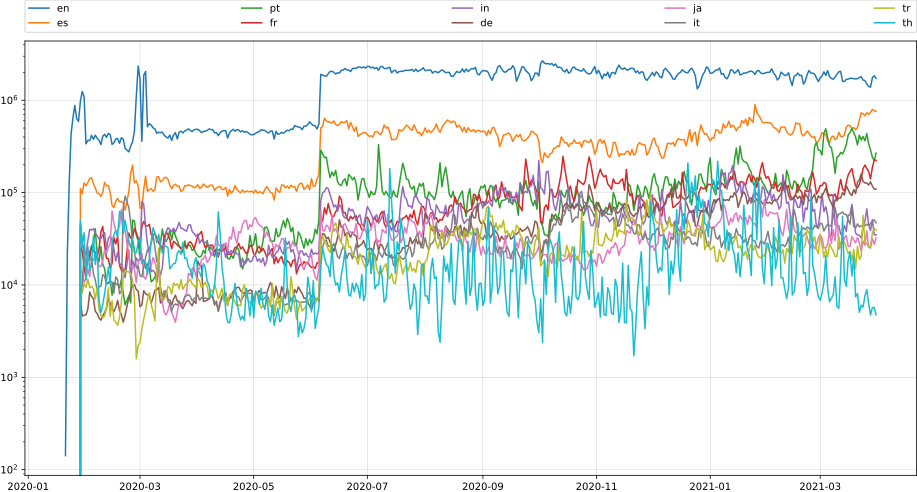
\includegraphics[scale=.4]{tweets_per_language_over_time}
    	\caption{Number of tweets over time for the top 10 languages}
    	\label{fig:tweets-language-over-time}
\end{figure}

\section{How to retrieve the data}
\label{sec:retrieve-data}

To comply with Twitter's terms of service,\footnote{\url{https://developer.twitter.com/en/developer-terms/agreement-and-policy}} tweets cannot be released publicly: the repository is in fact a collection of Tweet-IDs.

The original tweets can be retrieved, or \textit{hydrated}, using the Python library Twarc with a Twitter Developer Account. In fact, to be able to use the Twitter API, it is mandatory to apply to Twitter Developer.\footnote{\url{https://developer.twitter.com/en/apply-for-access}} When the application has been accepted, the developer will be entitled to access the API using tokens. 

Given the id of a tweet, Twarc uses the tokens of the associated developer account to contact the API, and returns the corresponding information as a json object. However, Twarc also tries to maximize the number of possible IDs per request and, at the same time, makes sure to be compliant with the API usage limits.

In the case of this dataset, the data came along with a script to hydrate the tweets automatically to facilitate the procedure.

\section{Tweets}
\label{sec:tweets}
The structure of the json object for the associated tweet depends on the version of the API used: for this project, we have used Standard v1.1 to hydrate the tweets.\footnote{\url{https://developer.twitter.com/en/docs/twitter-api/v1/data-dictionary/object-model/tweet}}

In general, a tweet is characterized by a number of different fields. For the scope of the project, we decided to keep only the most relevant fields, such as:

\begin{itemize}
	\item \texttt{id}, the integer representation of the unique identifier for this Tweet
	\item \texttt{created\_at}, UTC time when this Tweet was created
	\item \texttt{full\_text}, the actual UTF-8 text of the status update (not truncated)
	\item \texttt{user}, the user who posted this Tweet
	\item \texttt{retweeted\_status}, the presence of this attribute distinguishes Retweets from typical Tweets
	\item \texttt{favorite\_count}, indicates approximately how many times this Tweet has been liked by Twitter users
	\item \texttt{retweet\_count}, number of times this Tweet has been retweeted
	\item \texttt{lang}, indicates a BCP 47 language identifier corresponding to the machine-detected language of the Tweet text, or und if no language could be detected
\end{itemize}

Further information about the user that posted the tweet are available in the \texttt{user} field, such as:

\begin{itemize}
	\item \texttt{id}, the integer representation of the unique identifier for this User
	\item \texttt{name}, the name of the user, as they have defined it
	\item \texttt{screen\_name}, the screen name, handle, or alias that this user identifies themselves with
	\item \texttt{location}, the user-defined location for this account's profile. Not necessarily a location, nor machine-parseable
	\item \texttt{description}, the user-defined UTF-8 string describing their account
	\item \texttt{default\_profile\_image}, when true, indicates that the user has not uploaded their own profile image and a default image is used instead
	\item \texttt{profile\_image\_url\_https}, a HTTPS-based URL pointing to the user's profile image
	\item \texttt{followers\_count}, the number of followers this account currently has
	\item \texttt{statuses\_count}, the number of Tweets (including retweets) issued by the user
\end{itemize}

Given that, each json object associated with a tweet can be represented as follows:

\begin{lstlisting}[language=json, caption={Final json object for a Tweet}, captionpos=b, label={lst:tweet_json}]
{
  "id": 1307025659294674945,
  "full_text": "Here's an article that highlights the updates...",
  "lang": "en",
  "created_at": "Fri Sep 18 18:36:15 +0000 2020",
  "retweet_count": 11,
  "favorite_count": 70,
  "user": {
    "id": 2244994945,
    "id_str": "2244994945",
    "screen_name": "TwitterDev",
    "name": "Twitter Dev",
    "description": "The voice of the #TwitterDev team and your official...",
    "location": "127.0.0.1",
    "followers_count": 513958,
    "statuses_count": 3635,
    "default_profile_image": false,
    "profile_image_url_https": "https:\/\/pbs.twimg.com\/profile_images\/1283786620521652229\/lEODkLTh_normal.jpg"
  }
}
\end{lstlisting}



